% Options for packages loaded elsewhere
\PassOptionsToPackage{unicode}{hyperref}
\PassOptionsToPackage{hyphens}{url}
%
\documentclass[
  american,
  man,floatsintext]{apa7}
\usepackage{amsmath,amssymb}
\usepackage{lmodern}
\usepackage{ifxetex,ifluatex}
\ifnum 0\ifxetex 1\fi\ifluatex 1\fi=0 % if pdftex
  \usepackage[T1]{fontenc}
  \usepackage[utf8]{inputenc}
  \usepackage{textcomp} % provide euro and other symbols
\else % if luatex or xetex
  \usepackage{unicode-math}
  \defaultfontfeatures{Scale=MatchLowercase}
  \defaultfontfeatures[\rmfamily]{Ligatures=TeX,Scale=1}
\fi
% Use upquote if available, for straight quotes in verbatim environments
\IfFileExists{upquote.sty}{\usepackage{upquote}}{}
\IfFileExists{microtype.sty}{% use microtype if available
  \usepackage[]{microtype}
  \UseMicrotypeSet[protrusion]{basicmath} % disable protrusion for tt fonts
}{}
\makeatletter
\@ifundefined{KOMAClassName}{% if non-KOMA class
  \IfFileExists{parskip.sty}{%
    \usepackage{parskip}
  }{% else
    \setlength{\parindent}{0pt}
    \setlength{\parskip}{6pt plus 2pt minus 1pt}}
}{% if KOMA class
  \KOMAoptions{parskip=half}}
\makeatother
\usepackage{xcolor}
\IfFileExists{xurl.sty}{\usepackage{xurl}}{} % add URL line breaks if available
\IfFileExists{bookmark.sty}{\usepackage{bookmark}}{\usepackage{hyperref}}
\hypersetup{
  pdftitle={Study 2},
  pdfauthor={Blinded1, Blinded2, Blinded1, \& Blinded1},
  pdflang={en-US},
  pdfkeywords={keywords},
  hidelinks,
  pdfcreator={LaTeX via pandoc}}
\urlstyle{same} % disable monospaced font for URLs
\usepackage{graphicx}
\makeatletter
\def\maxwidth{\ifdim\Gin@nat@width>\linewidth\linewidth\else\Gin@nat@width\fi}
\def\maxheight{\ifdim\Gin@nat@height>\textheight\textheight\else\Gin@nat@height\fi}
\makeatother
% Scale images if necessary, so that they will not overflow the page
% margins by default, and it is still possible to overwrite the defaults
% using explicit options in \includegraphics[width, height, ...]{}
\setkeys{Gin}{width=\maxwidth,height=\maxheight,keepaspectratio}
% Set default figure placement to htbp
\makeatletter
\def\fps@figure{htbp}
\makeatother
\setlength{\emergencystretch}{3em} % prevent overfull lines
\providecommand{\tightlist}{%
  \setlength{\itemsep}{0pt}\setlength{\parskip}{0pt}}
\setcounter{secnumdepth}{-\maxdimen} % remove section numbering
% Make \paragraph and \subparagraph free-standing
\ifx\paragraph\undefined\else
  \let\oldparagraph\paragraph
  \renewcommand{\paragraph}[1]{\oldparagraph{#1}\mbox{}}
\fi
\ifx\subparagraph\undefined\else
  \let\oldsubparagraph\subparagraph
  \renewcommand{\subparagraph}[1]{\oldsubparagraph{#1}\mbox{}}
\fi
% Manuscript styling
\usepackage{upgreek}
\captionsetup{font=singlespacing,justification=justified}

% Table formatting
\usepackage{longtable}
\usepackage{lscape}
% \usepackage[counterclockwise]{rotating}   % Landscape page setup for large tables
\usepackage{multirow}		% Table styling
\usepackage{tabularx}		% Control Column width
\usepackage[flushleft]{threeparttable}	% Allows for three part tables with a specified notes section
\usepackage{threeparttablex}            % Lets threeparttable work with longtable

% Create new environments so endfloat can handle them
% \newenvironment{ltable}
%   {\begin{landscape}\begin{center}\begin{threeparttable}}
%   {\end{threeparttable}\end{center}\end{landscape}}
\newenvironment{lltable}{\begin{landscape}\begin{center}\begin{ThreePartTable}}{\end{ThreePartTable}\end{center}\end{landscape}}

% Enables adjusting longtable caption width to table width
% Solution found at http://golatex.de/longtable-mit-caption-so-breit-wie-die-tabelle-t15767.html
\makeatletter
\newcommand\LastLTentrywidth{1em}
\newlength\longtablewidth
\setlength{\longtablewidth}{1in}
\newcommand{\getlongtablewidth}{\begingroup \ifcsname LT@\roman{LT@tables}\endcsname \global\longtablewidth=0pt \renewcommand{\LT@entry}[2]{\global\advance\longtablewidth by ##2\relax\gdef\LastLTentrywidth{##2}}\@nameuse{LT@\roman{LT@tables}} \fi \endgroup}

% \setlength{\parindent}{0.5in}
% \setlength{\parskip}{0pt plus 0pt minus 0pt}

% Overwrite redefinition of paragraph and subparagraph by the default LaTeX template
% See https://github.com/crsh/papaja/issues/292
\makeatletter
\renewcommand{\paragraph}{\@startsection{paragraph}{4}{\parindent}%
  {0\baselineskip \@plus 0.2ex \@minus 0.2ex}%
  {-1em}%
  {\normalfont\normalsize\bfseries\itshape\typesectitle}}

\renewcommand{\subparagraph}[1]{\@startsection{subparagraph}{5}{1em}%
  {0\baselineskip \@plus 0.2ex \@minus 0.2ex}%
  {-\z@\relax}%
  {\normalfont\normalsize\itshape\hspace{\parindent}{#1}\textit{\addperi}}{\relax}}
\makeatother

% \usepackage{etoolbox}
\makeatletter
\patchcmd{\HyOrg@maketitle}
  {\section{\normalfont\normalsize\abstractname}}
  {\section*{\normalfont\normalsize\abstractname}}
  {}{\typeout{Failed to patch abstract.}}
\patchcmd{\HyOrg@maketitle}
  {\section{\protect\normalfont{\@title}}}
  {\section*{\protect\normalfont{\@title}}}
  {}{\typeout{Failed to patch title.}}
\makeatother
\keywords{keywords\newline\indent Word count: TBC}
\usepackage{csquotes}
\ifxetex
  % Load polyglossia as late as possible: uses bidi with RTL langages (e.g. Hebrew, Arabic)
  \usepackage{polyglossia}
  \setmainlanguage[variant=american]{english}
\else
  \usepackage[main=american]{babel}
% get rid of language-specific shorthands (see #6817):
\let\LanguageShortHands\languageshorthands
\def\languageshorthands#1{}
\fi
\ifluatex
  \usepackage{selnolig}  % disable illegal ligatures
\fi
\newlength{\cslhangindent}
\setlength{\cslhangindent}{1.5em}
\newlength{\csllabelwidth}
\setlength{\csllabelwidth}{3em}
\newenvironment{CSLReferences}[2] % #1 hanging-ident, #2 entry spacing
 {% don't indent paragraphs
  \setlength{\parindent}{0pt}
  % turn on hanging indent if param 1 is 1
  \ifodd #1 \everypar{\setlength{\hangindent}{\cslhangindent}}\ignorespaces\fi
  % set entry spacing
  \ifnum #2 > 0
  \setlength{\parskip}{#2\baselineskip}
  \fi
 }%
 {}
\usepackage{calc}
\newcommand{\CSLBlock}[1]{#1\hfill\break}
\newcommand{\CSLLeftMargin}[1]{\parbox[t]{\csllabelwidth}{#1}}
\newcommand{\CSLRightInline}[1]{\parbox[t]{\linewidth - \csllabelwidth}{#1}\break}
\newcommand{\CSLIndent}[1]{\hspace{\cslhangindent}#1}

\title{Study 2}
\author{Blinded\textsuperscript{1}, Blinded\textsuperscript{2}, Blinded\textsuperscript{1}, \& Blinded\textsuperscript{1}}
\date{}


\shorttitle{Cognitive Load and Moral Dumbfounding}

\authornote{

Correspondence concerning this article should be addressed to Blinded, Blinded. E-mail: Blinded

}

\affiliation{\vspace{0.5cm}\textsuperscript{1} Blinded\\\textsuperscript{2} Blinded}

\abstract{
Six studies etc.
}



\begin{document}
\maketitle

\hypertarget{study-2---online-replication-1}{%
\section{Study 2 - Online Replication 1}\label{study-2---online-replication-1}}

Study 1 demonstrated interesting variability in responses to the critical slide depending on cognitive load. The aim of Study 2 was to assess the replicability of the results of Study 1, using an online sample. In Study 1, the experimenter was in the room with the participants. This made it more difficult for participants to cheat on the memory task. This is not possible with an online sample. An alternative cognitive load manipulation was taken from De Neys and Schaeken (De Neys \& Schaeken, 2007), whereby a dot pattern is briefly presented to participants, and participants are required to reproduce the dot pattern at a later stage.

\hypertarget{study-2-method}{%
\subsection{Study 2: Method}\label{study-2-method}}

\hypertarget{study-2-participants-and-design}{%
\subsubsection{Study 2: Participants and design}\label{study-2-participants-and-design}}

Study 2 was a between subjects design. The dependent variable was response to the critical slide. The independent variable was cognitive load with two levels: high and low. Need for Cognition (Cacioppo \& Petty, 1982; Petty, Cacioppo, \& Kao, 1984) was included as a potential correlate and moderator variable.

A total sample of 100 participants (56 female, 44 male; \emph{M}\textsubscript{age} = 38.38, min = 19, max = 72, \emph{SD} = 12.41) took part. Participants in this sample were recruited using Amazon's MTurk (Amazon Web Services Inc., 2016). Participants were paid \$0.50 for their participation. Participants were recruited from English speaking countries or from countries where residents generally have a high level of English (e.g., The Netherlands, Denmark, Sweden).

\hypertarget{study-2-procedure-and-materials}{%
\subsubsection{Study 2: Procedure and materials}\label{study-2-procedure-and-materials}}

Data were collected using an online questionnaire. Materials were largely the same as in Study 1, with a change to the cognitive load manipulation. Cognitive load was manipulated using a dot-pattern memory task (De Neys \& Schaeken, 2007).

Participants were presented with a 3 x 3 grid containing a dot pattern. This image disappeared after one second. Participants then answered a question relating to the moral judgement task. Following this, participants were asked to reproduce the dot-pattern. All participants took part in the memory task, and cognitive load was manipulated by varying the complexity of the patterns presented (De Neys \& Schaeken, 2007). The control group were presented with simple patterns, containing three dots in a line, while the experimental group were presented with more complex dot patterns containing 4 dots, see Figure~\ref{fig:S2dotpattern}.

\begin{figure}
\centering
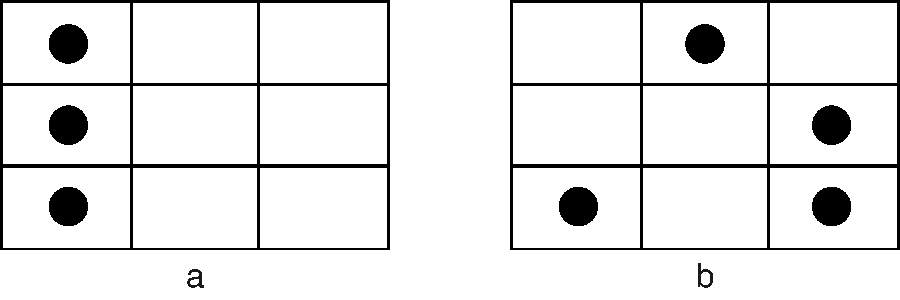
\includegraphics{Study_2_files/figure-latex/S2dotpattern-1.pdf}
\caption{\label{fig:S2dotpattern}Sample dot patterns - more simple for the control group (a) and higher complexity for the experimental condition (b)}
\end{figure}

Study 2 proceeded in much the same way as Study 1. There were four target questions during which participants were engaged in the memory task. A different pattern was presented before each of the following: the initial judgement, the initial opportunity to provide reasons, the critical slide, and the revised judgement. After each of these questions participants were required to reproduce the pattern. As in Study 1, dumbfounding was measured using the critical slide.

\hypertarget{study-2-results}{%
\subsection{Study 2: Results}\label{study-2-results}}

Seventy seven participants (77\%) rated the behavior of Julie and Mark as wrong initially, and seventy participants (70\%) rated the behavior as wrong at the end of the task. Initial ratings (\emph{M} = 2.13, \emph{SD} = 1.54) were significantly more severe than revised ratings (\emph{M} = 2.35, \emph{SD} = 1.65), \emph{t}(99) = -2.85, \emph{p} = .005; \emph{d} = 0.28. Inspection of the binned judgments revealed that ten participants changed the valence of their judgments, and all but one of these involved one judgment that was neutral (see Supplementary materials Table XX).

Participants who selected the admission of not having reasons on the critical slide were identified as dumbfounded. Twenty six participants (26\%) selected ``It's wrong but I can't think of a reason.'' Fifty participants (50\%) selected ``It's wrong and I can provide a valid reason''; and twenty four participants (24\%) selected ``There is nothing wrong.''

A chi-squared test for independence revealed no association between experimental condition and response to the critical slide, \(\chi\)\textsuperscript{2}(2, \emph{N} = 100) = 0.74, \emph{p} = .690, \emph{V} = 0.09, the observed power was 0.11. The responses to the critical slide for the experimental group (\emph{N} = 51) and the control group (\emph{N} = 49) are displayed in Figure~\ref{fig:S2figboth}.

\begin{figure}
\centering
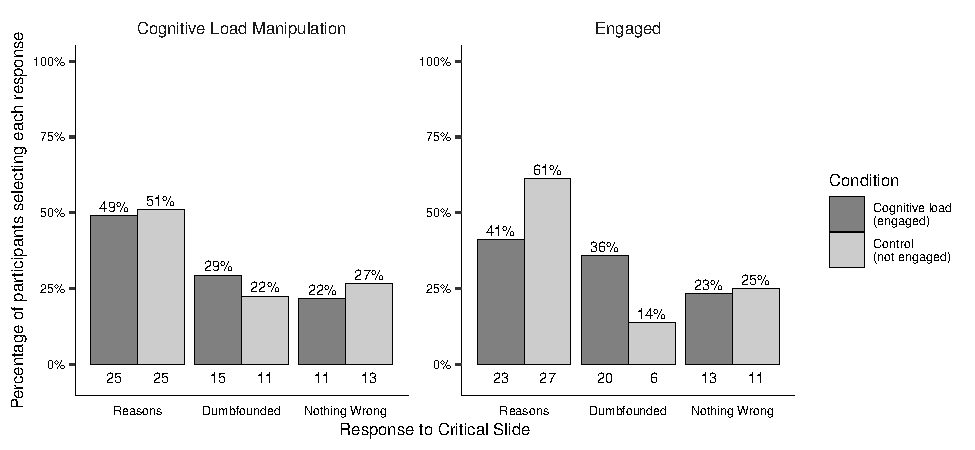
\includegraphics{Study_2_files/figure-latex/S2figboth-1.pdf}
\caption{\label{fig:S2figboth}Study 2: Responses to critical slide for (left) the experimental group (\emph{N} = 51) vs the control group (\emph{N} = 49); and (right) depending on engagement (\emph{N} = 56) or non-engagement (\emph{N} = 44) with the memory task}
\end{figure}

It is possible that the difference in results observed between Study 1 and Study 2 is due to the alternative manipulation of cognitive load employed. In Study 1, the control group did not engage in any task, however, adopting De Neys and Shaeken's procedure (2007), participants in the control group of Study 2 engaged in a memory task. It is possible that simply engaging in a memory task led to differences in responses, and that level of difficulty (the manipulation that was employed) was irrelevant. Indeed, the responding to the critical slide in the control group in Study 2 is more similar to the responding in the experimental group in 1 than to the control group in Study 1. Furthermore, rates of successful reproduction of the dot patterns in Study 2 were much lower than reported by De Neys and Shaeken (2007). It is likely that engagement with the memory task in Study 2 was not comparable to that observed by De Neys and Shaeken (2007), and this impacted the results. We propose that not engaging appropriately with the memory task undermines its efficacy as a cognitive load manipulation, and hypothesized that the effect of the cognitive load manipulation is related to the degree to which people engage with the manipulation.

\begin{table}[tbp]

\begin{center}
\begin{threeparttable}

\caption{\label{tab:S2S2tab1dumb}Study 2 – Observed counts, expected counts, and standardised residuals for each response to the critical slide depending on cognitive load}

\begin{tabular}{llcc}
\toprule
 & \multicolumn{1}{c}{} & \multicolumn{1}{c}{Engaged} & \multicolumn{1}{c}{Not Engaged}\\
\midrule
Observed count & Reasons & 23 & 27\\
 & Dumbfounded & 20 & 6\\
 & Nothing Wrong & 13 & 11\\
Expected count & Reasons & 28 & 22\\
 & Dumbfounded & 14.56 & 11.44\\
 & Nothing Wrong & 13.44 & 10.56\\
Standardised residuals & Reasons & -2.01* & 2.01*\\
 & Dumbfounded & 2.5* & -2.5*\\
 & Nothing Wrong & -0.21 & 0.21\\
\bottomrule
\addlinespace
\end{tabular}

\begin{tablenotes}[para]
\normalsize{\textit{Note.} * = sig. at \emph{p} < .05; ** = sig. at \emph{p} < .001}
\end{tablenotes}

\end{threeparttable}
\end{center}

\end{table}

To test this claim we developed a measure of engagement with the memory task. The memory task involved correctly placing dots in a 3 x 3 grid. For the scoring of this task, each of the nine places in the grid could be marked/not marked correctly or incorrectly, making 9 the total possible number of correct responses. If a person misplaced one dot in the pattern this would count for 2 incorrect places in the grid: the mark in the incorrect place, and the absence of a mark in the place it should have been. A participant who received a score of 7, could reasonably be taken to have engaged with the task, and simply made a slip. As such, this was taken as the cut-off point for identifying engagement. This resulted in 56 participants being identified as engaging with the memory task, and 44 being identified as not engaging with the task.

Using this engagement threshold, we tested if responses to the critical were associated with engagement with the memory task. A chi-squared test for independence revealed an association between engagement in the memory task and response to the critical slide, \(\chi\)\textsuperscript{2}(2, \emph{N} = 100) = 6.68, \emph{p} = .035, \emph{V} = 0.26, the observed power was 0.11. The responses to the critical slide for the experimental group (\emph{N} = 51) and the control group (\emph{N} = 49) are displayed in Figure~\ref{fig:S2figboth}. The observed counts, expected counts and standardized residuals are displayed in Table~\ref{tab:S2S2tab1dumb}.

A multinomial logistic regression revealed no significant association between Need for Cognition and response to the critical slide, \(\chi\)\textsuperscript{2}(2, \emph{N} = 100) = 2.19, \emph{p} = .334, the observed power was 0.24 (see supplementary Figure XX for relative probabilities of selecting each response depending on Need for Cognition).

\hypertarget{refs}{}
\begin{CSLReferences}{1}{0}
\leavevmode\hypertarget{ref-amazonwebservicesinc._amazon_2016}{}%
Amazon Web Services Inc. (2016). \emph{Amazon {Mechanical Turk}}.

\leavevmode\hypertarget{ref-cacioppo_need_1982}{}%
Cacioppo, J. T., \& Petty, R. E. (1982). The need for cognition. \emph{Journal of Personality and Social Psychology}, \emph{42}(1), 116--131. \url{https://doi.org/10.1037/0022-3514.42.1.116}

\leavevmode\hypertarget{ref-deneys_when_2007}{}%
De Neys, W., \& Schaeken, W. (2007). When people are more logical under cognitive load: Dual task impact on scalar implicature. \emph{Experimental Psychology}, \emph{54}(2), 128--133. \url{https://doi.org/10.1027/1618-3169.54.2.128}

\leavevmode\hypertarget{ref-petty_efficient_1984}{}%
Petty, R. E., Cacioppo, J. T., \& Kao, C. F. (1984). The efficient assessment of need for cognition. \emph{Journal of Personality Assessment}, \emph{48}(3), 306--307.

\end{CSLReferences}


\end{document}
